\chapter{Task Distribution in a Flat Organization\label{sec:work-distribution}}
\chaptermark{Task Distribution}

\iftoggle{glossarysubstitutionworks}{\Gls{bureaucracy}}{Bureaucracy}  
forms part of the explanation for patterns observed when people interact. Another explanatory aspect is how tasks get distributed among members of an organization. These two aspects of participating in an organization are often confounded. This chapter describes a model of processes and tasks that involve coordination. 
The model is useful for distinguishing the effects of bureaucracy (distributed knowledge and distributed decision-making) from the distribution of tasks in an organization.

The model of task distribution in an organization is sufficiently detailed to illustrate commonly observed situations but is agnostic to the specific tasks or work roles. Improvements to the model intended to increase the realism could be made, but risk decreasing the clarity of the model.

\section{Assumptions in the Model of Task Distribution}

The model relies on a few concepts. These definitions are local to the numerical model and do not apply to the rest of the book:
\begin{itemize}
    \item \textbf{Specialization}: categories of ability. A person has a specialization. Completing a task is associated with a specialization.
    \item \textbf{Skill-level}: a ranking of how quickly work can be done for a task. If a task requires a skill-level higher than a person has, then that person is unable to complete the task.
    \item \textbf{Person}: is a member of the organization, has specializations, has a skill-level per specialization, can receive tasks, and can engage with other people in the organization. A person can complete one task at a time. A person can coordinate one task at a time. A person has the following attributes:
    \begin{itemize}
        \item Person's contact list: A person has a list of people they've previously given tasks to. When figuring out who to give a task to, they can review the list of people they already know. 
        \item Person's backlog: Each person maintains a queue of tasks to be done.
        \item Person's status: A person is either idle (not assigned a task), working on a task, or coordinating with other people. 
    \end{itemize}
    \item \textbf{Organization}: a set of people who can be assigned tasks to work on. 
    \item Task: requires one specialization, has an associated minimum skill-level, and has an amount of time that the task takes. A task can only be worked on by one person at a time. 
    \item \textbf{Process}: comprised of one or more tasks.\footnote{See Wikipedia entry on 
    \index{Wikipedia!\href{https://en.wikipedia.org/wiki/Queueing_theory}{Queueing Theory}}
    \href{https://en.wikipedia.org/wiki/Queueing_theory}{Queueing Theory}.} Tasks in a process are worked on sequentially by people. At any given time the process is owned by one person who is either coordinating or working on the task.  Processes are independent.
\end{itemize}

In the model I'm using the word task instead of work because work is a Physics concept that applies when there is a product that is tangible and countable. Making tacos takes work; approving requests is a distinct concept because there is nothing tangible. For knowledge workers, which most bureaucrats are, the unit of tasking is attention-time spent on an issue.
Each participant in the organization has the same amount of attention-time to spend, but different specializations and skill-levels per specialization.

%The model is abstract so that is applicable to many contexts. 
%A simple process is a sequence of few tasks, and each task does not require significant specialization or skill-level.
%A complex process is a sequence of many tasks, and each task requires specialized skills, and the number of distinct specializations is high.

When a person is assigned a task they don't have the specialization for or lack sufficient skill-level in that specialization, then they have to find someone else in the organization who is capable of doing the task. 
In the numerical model the random selection of someone else who has the necessary specialization and skill-level is insensitive to the size of their backlog. This reflects my experience in  large organizations where task backlogs are not visible. As a consequence, you merely add something to their backlog and hope they will get to it eventually.



The model relies on a process being a sequence of tasks. That might not be realistic when branching is part of a process (conditional branching or splitting).
Real processes feature branching in two senses. The first sense of branching is the conditional logic: ``if this else that.''
The second sense of branching is that a task is the initiation point of another process. 
In either of those two senses of branching the processes can be treated as independent sequences of tasks.



Simplifying assumptions about what isn't in the numerical model:
\begin{itemize}
    \item There is nothing in the model about policies, decision making~\cite{2009_Klimek}, shared resources, or subjects of bureaucracy. This model is included in a book about bureaucracy to show that not all patterns observed in an organization should be blamed on bureaucracy. 
    \item There's no hierarchy in the model. The model assumes people are cooperating in the organization. Unlike the rest of the book, this model does not use the distinction of organizations being comprised of teams.
    \item People in the model don't get to initiate tasks of their own volition. They work on tasks that are either from their personal backlog or from an infinite set of tasks.
    \item People in the model don't get to refuse any task that is assigned to them for which they have the specialization and relevant skill-level.
    \item No overtime. Every person gets the same amount of time to do work.
    \item No support staff. All infrastructure for communication and tasks works without failure.
    \item No dark patterns. Everyone does the task assigned promptly and correctly.
    \item No turnover of staff during the simulation.
    \item No improvement of skill-level per person, or added specialization.
\end{itemize}
The complexities above are not included in the model because the point of the model is to show what arises from simple constraints. 

Within the constraints, improvements could be made to the model.  %, but are not expected to alter the conclusions:
However,  conclusions drawn from the model map to real-world organizations even without these features: 
\begin{itemize}
    \item Use realistic distributions (e.g., power law) instead of uniform distributions.
    \item When a person is not qualified to do a task, instead of searching randomly, search second-order contacts.
\end{itemize}

\section{Examples of Tasks and People}

Suppose the model is configured to simulate three specializations (A, B, C) and three skill-levels (1, 2, 3). 

\subsection*{Example People\label{sec:example-people}}

A person with skill-level 3 in specialization A and skill-level 1 in specialization C is labeled ``A3,C1''. A visualization of their capabilities is the following table:

\begin{center}
\begin{tabular}{c|c|c|c|}
&\multicolumn{3}{c}{\footnotesize Specializations}\\
\hline
& A & B & C \\
\hline
1 & X & & X \\
\hline
2 & X & & \\
\hline
3 & X & & \\
\hline
\end{tabular}
\end{center}

Because this person has skill-level three in specialization A, that means they can also work on tasks that require skill-level two or skill-level one.

People can be characterized by the depth and breadth of their skills. For example, a ``expert specialist'' (e.g.,~``B3") is good at one thing, while a ``general specialist" (e.g.,~``A1,B3,C1") has \href{https://en.wikipedia.org/wiki/T-shaped_skills}{T-shaped skills}:

\begin{center}
Expert:
$\left\{
\begin{tabular}{c|c|c|c|}
&\multicolumn{3}{c}{\footnotesize Specializations}\\
%\hline
& A & B & C \\
\cline{2-4}
1 & &  X &  \\
\cline{2-4}
2 & & X & \\
\cline{2-4}
3 & & X & \\
\cline{2-4}
\end{tabular}
\right.$
\qquad
Generalist Expert:
$\left\{
\begin{tabular}{c|c|c|c|}
& \multicolumn{3}{c}{\footnotesize Specializations}\\
%\hline
& A & B & C \\
\cline{2-4}
1 & X &  X & X \\
\cline{2-4}
2 & & X & \\
\cline{2-4}
3 & & X & \\
\cline{2-4}
\end{tabular}
\right.$
\end{center}

A generalist (here~``A1,B1,C1") is not an expert at anything but is capable in multiple specializations. A unicorn (here~``A3,B3,C3") can do everything well.
\begin{center}
Generalist:
$\left\{
\begin{tabular}{c|c|c|c|}
 & \multicolumn{3}{c}{\footnotesize Specializations}\\
%\hline
& A & B & C \\
\cline{2-4}
1 & X &  X & X \\
\cline{2-4}
 2 & &  & \\
\cline{2-4}
3 &  &  & \\
\cline{2-4}
\end{tabular}
\right.$
\qquad
Unicorn:
$\left\{
\begin{tabular}{c|c|c|c|}
& \multicolumn{3}{c}{\footnotesize Specializations}\\
%\hline
   & A & B & C \\
\cline{2-4}
 1 & X & X & X \\
\cline{2-4}
 2 & X & X & X \\
\cline{2-4}
 3 & X & X & X \\
\cline{2-4}
\end{tabular}
\right.$
\end{center}


There are many more unskilled specialists (e.g.,~``A1'') than unicorns.
\begin{center}
Unskilled Specialist:
$\left\{
\begin{tabular}{c|c|c|c|}
& \multicolumn{3}{c}{\footnotesize Specializations}\\
%\hline
   & A & B & C \\
\cline{2-4}
 1 & X &   &  \\
\cline{2-4}
 2 &   &   & \\
\cline{2-4}
 3 &   &   & \\
\cline{2-4}
\end{tabular}
\right.$
\end{center}

\subsection*{Tasks and Processes}

A task that requires skill-level 2 in specialization B is labeled ``B2.''
%\begin{center}
%\begin{tabular}{|c|c|c|}
%\multicolumn{3}{c}{\footnotesize Specializations}\\
%\hline
%A & B & C \\
%\hline
% &   &  \\
%\hline
% & X & \\
%\hline
% & & \\
%\hline
%\end{tabular}
%\end{center}
The assumption that a task requires one specialization is based on the idea that a process can be broken into atomic units. 

If a task requires skill-level 2 and takes 10 minutes, then
\begin{itemize}
    \item A person with skill-level 2 completes the task in 10 minutes.
    \item A person with skill-level 3 completes the task in  7 minutes (=10/(3/2)).
    \item A person with skill-level 1 is unable to complete the task.
\end{itemize}


A process is a sequence of tasks. For example, the list ``B2:10, A1:5, C3:7" describes three tasks: 
\begin{enumerate}
    \item Task requiring specialization B and skill-level 2; duration of 10 minutes.
    \item Task requiring specialization A and skill-level 1; duration of 5 minutes.
    \item Task requiring specialization C and skill-level 3; duration of 7 minutes.    
\end{enumerate}

\section{Configurations of the Task Distribution Model}

Comparing different configurations of the model requires a metric. 
Task throughput is a way to characterize the productivity of an organization. 


\subsection*{Scenario: Everyone is an A1}

Suppose every person in the organization is an A1 and every task is an A1.

\begin{center}
\begin{tabular}{c|c|}
%\cline{2}
  & A \\
\cline{2-2}
1 & X \\
\cline{2-2}
\end{tabular}
\end{center}

As a consequence of this configuration, no coordination is required because each person can do every task. Observations about this configuration include:
\begin{itemize}
    \item The number of people each person knows is irrelevant because coordination is unnecessary.
    \item This configuration yields the maximum throughput tasks for the organization.
    \item Adding more people increases the throughput.
\end{itemize}

These same conclusions hold for any configuration of an organization comprised of unicorns. 
The concept of every member being able to do any task is the model 
\index{Wikipedia!\href{https://en.wikipedia.org/wiki/Adhocracy}{adhocracy}}
\href{https://en.wikipedia.org/wiki/Adhocracy}{adhocracy} advocates. The feasibility of gathering people with relevant talents becomes challenging as the task complexity increases or increased throughput is needed. That is why organizations hire people who are not unicorns. 



%\subsection*{Scenario: A1,B1 or A1,B0 or A0,B1 or A0,B0\\with (task duration = coordination duration)\\with no social circle}
\subsection*{Scenario: A1,B1 or A1,B0 or A0,B1 or A0,B0}

The simplest non-trivial scenario occurs when not every member of an organization can do every task. For example, suppose  there are two specializations (A, B) and one skill level: 

\begin{center}
\begin{tabular}{c|c|c|}
%\cline{2-3}
  & A & B \\
\cline{2-3}
1 & X &   \\
\cline{2-3}
\end{tabular}
\quad and \quad
\begin{tabular}{c|c|c|}
%\cline{2-3}
  & A & B \\
\cline{2-3}
1 &   & X \\
\cline{2-3}
\end{tabular}
\quad and \quad
\begin{tabular}{c|c|c|}
%\cline{2-3}
  & A & B \\
\cline{2-3}
1 & X & X \\
\cline{2-3}
\end{tabular}
\quad and \quad
\begin{tabular}{c|c|c|}
%\cline{2-3}
  & A & B \\
\cline{2-3}
1 &   &   \\
\cline{2-3}
\end{tabular}
\end{center}
In this configuration, the person qualified as A1,B1 is labeled a unicorn -- they can do any task. Whether you consider inclusion of A0,B0 (a person who does no work and can only coordinate) to be relevant depends on your personal experience. Most organizations label these members as ``managers.'' 

When a person does not have all the specializations, then a task randomly assigned to one person may need to be given to someone else in the organization. For example, if I am an A1 and am given a B1 task, I need to find a coworker who is either qualified as B1 or A1,B1. Sharing tasks among members of the organization requires coordination.




\begin{figure}[H] % [!htb] %  https://tex.stackexchange.com/a/32605/235813
\centering
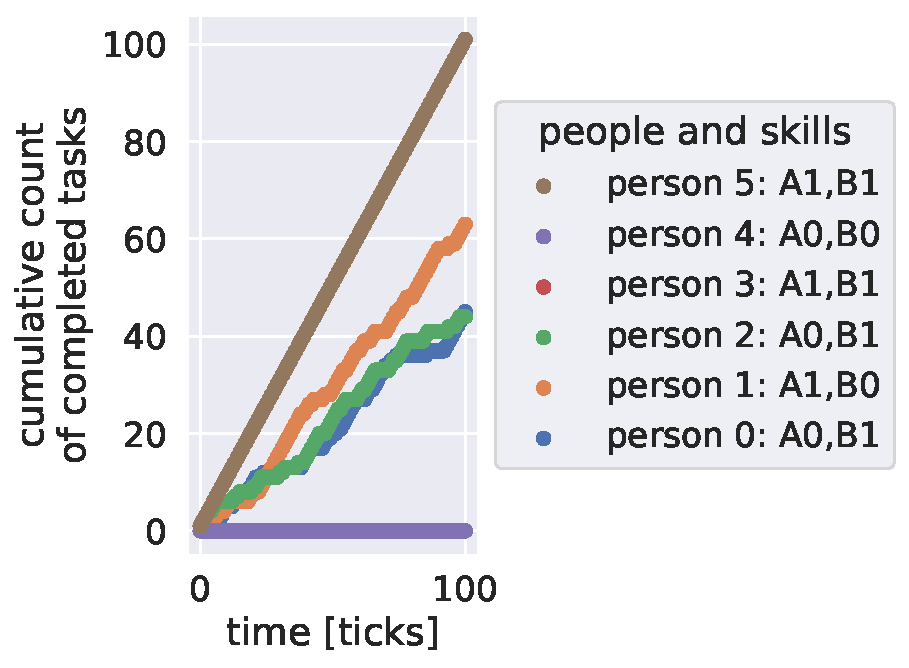
\includegraphics[width=1\textwidth]{images/task_distribution_tasks_per_person_simCount1_skills2_levels1_taskduration1_people6_social0_ticks100.pdf}
\caption{Tasks completed by each person in an organization with six people. Rather than count tasks per tick during steady-state, here we count the number of tasks completed in 100 ticks. Persons 3 and 5 both have the maximum throughput of tasks since they are unicorns. Person 0 has no throughput and only delegates tasks. Everyone is busy (no one is idle), but the level of productivity (tasks completed per time) varies.}
\label{fig:task-distribution-tasks-per-person}
\end{figure}



\begin{figure}[H] % [!htb]%  https://tex.stackexchange.com/a/32605/235813
\centering
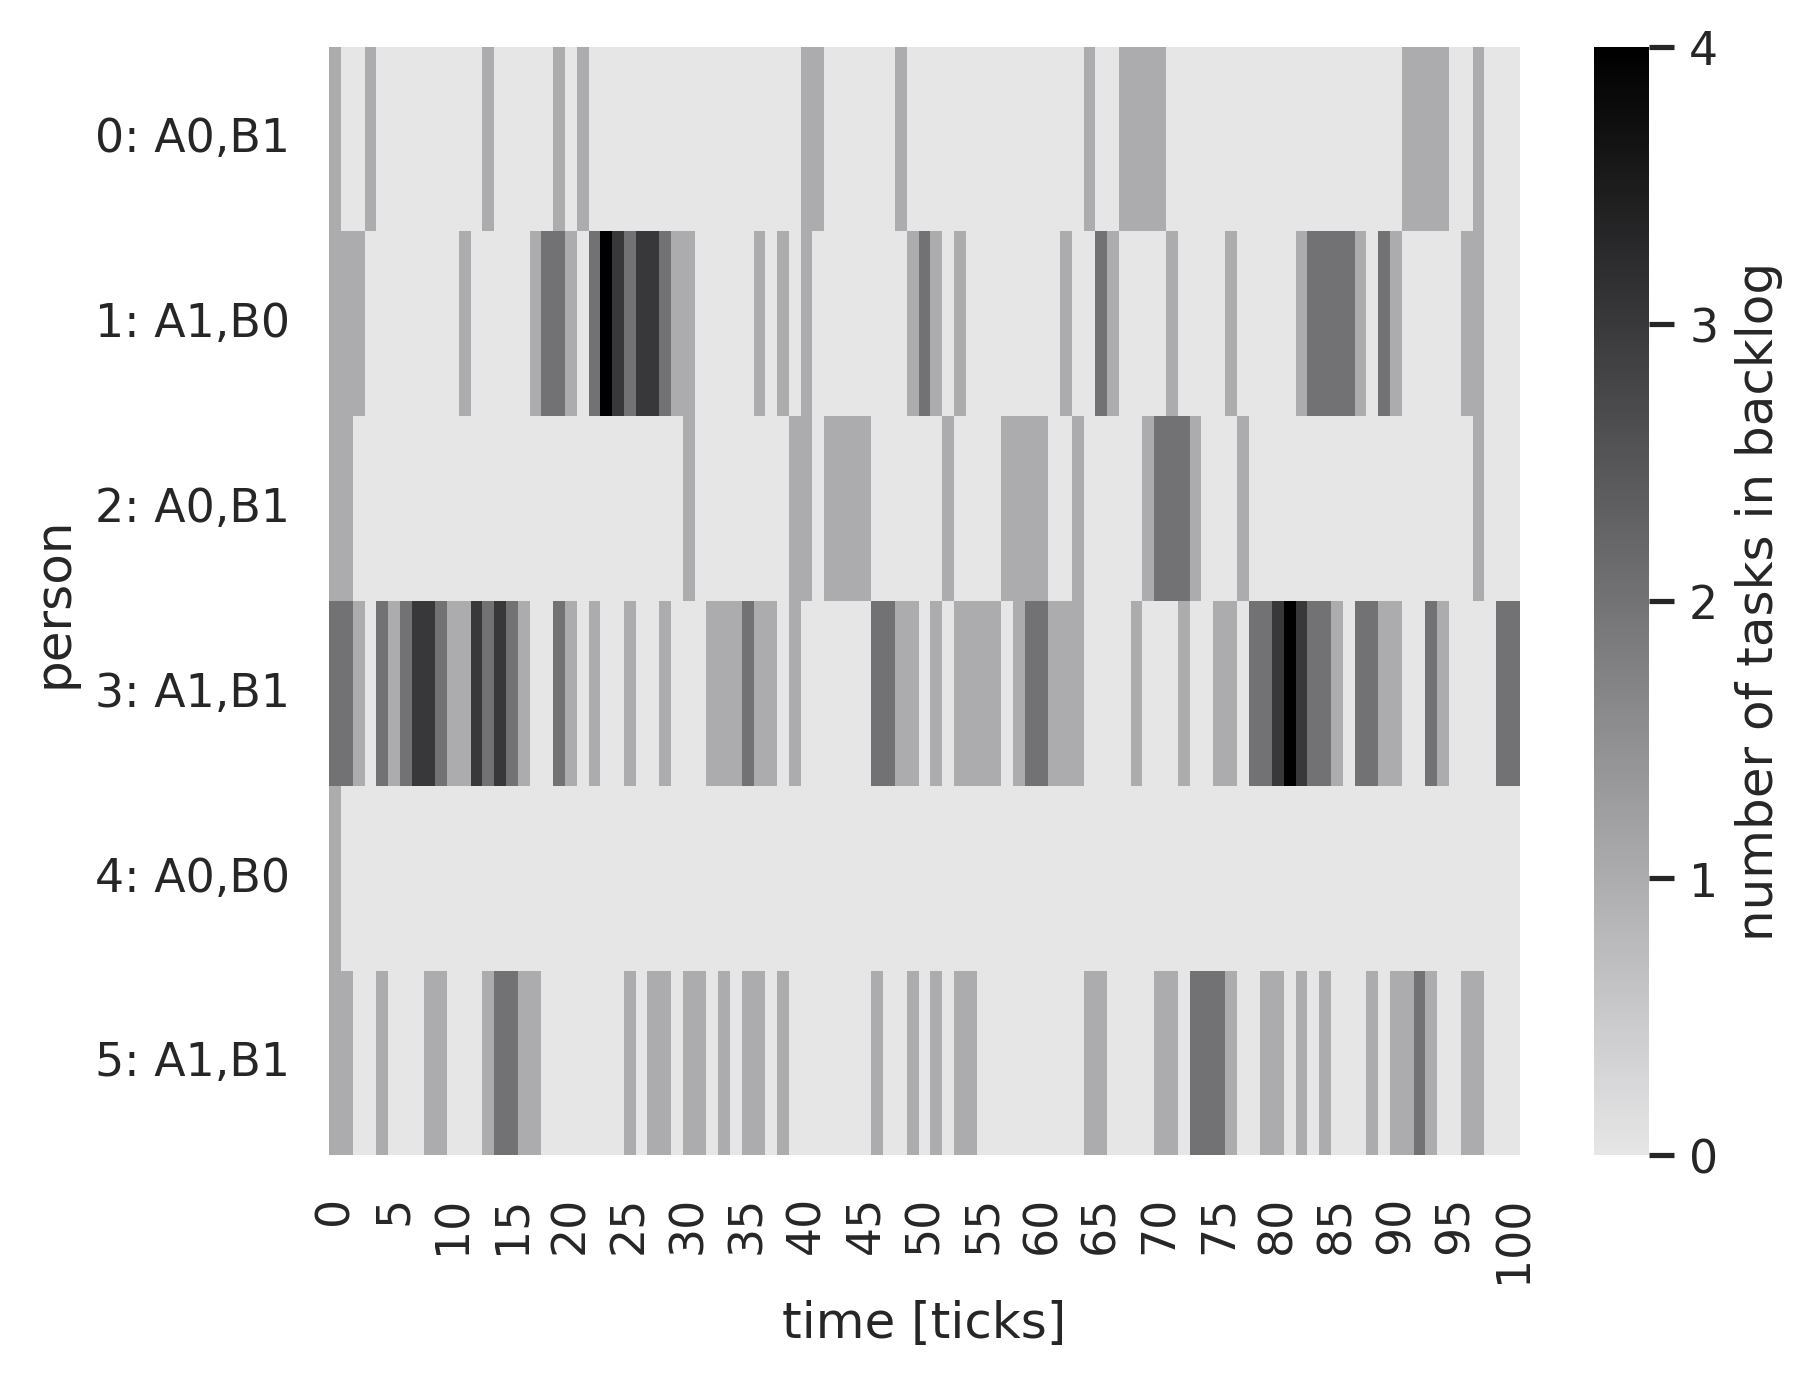
\includegraphics[width=1\textwidth]{images/task_distribution_backlog_length_per_person_simCount1_skills2_levels1_taskduration1_people6_social0_ticks100.png}
\caption{The length of each person's backlog (for the same six people) as a function of time. This is the same simulation as shown in Figure~\ref{fig:task-distribution-tasks-per-person}. The backlog of person 4 is empty because they are always delegating and no one assigns them tasks. Person 3 has a longer backlog because they are capable of doing any task.}
\label{fig:task-distribution-backlog-length}
\end{figure}





\begin{figure}[H] % [!htb] %  https://tex.stackexchange.com/a/32605/235813
\centering
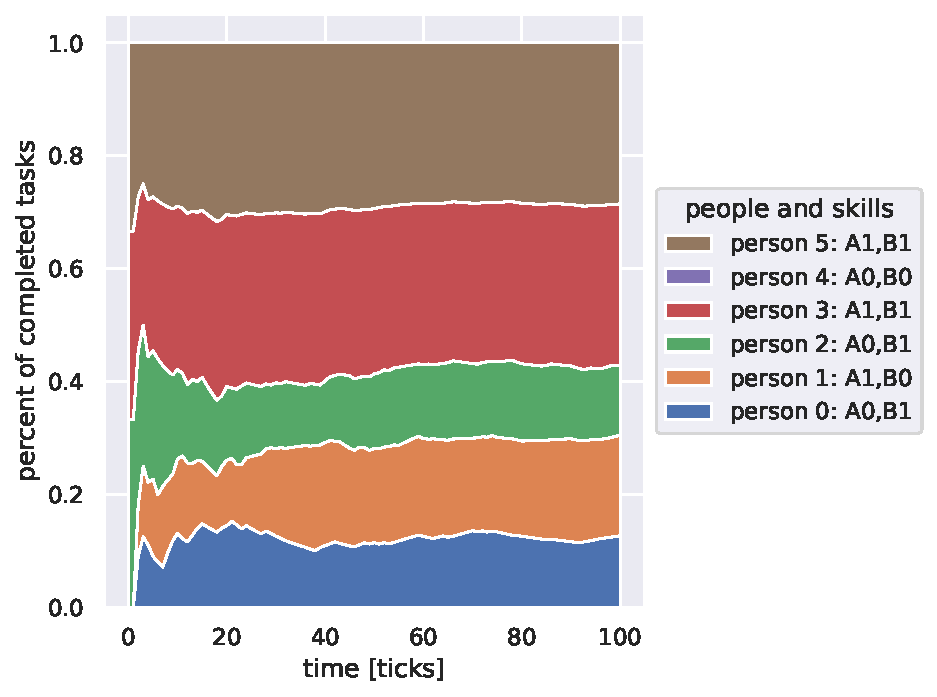
\includegraphics[width=1\textwidth]{images/task_distribution_percent_of_tasks_per_person_simCount1_skills2_levels1_taskduration1_people6_social0_ticks100.pdf}
\caption{This is the same simulation as shown in Figures~\ref{fig:task-distribution-tasks-per-person} and~\ref{fig:task-distribution-backlog-length}. The steady-state distribution emerges around 50 ticks. Person 3 and person 5 are both unicorns and have similar task throughput. Person 3 does not appear in this figure because they completed no tasks.}
\label{fig:task-distribution-percent-of-tasks}
\end{figure}



%a metric of interest is the number of task per simulated tick as a function of the number of people present in the organization.



The need for coordination can be blamed on the random delegation of tasks not being aligned to the specializations and skill-levels of the workers. 
The distribution of skills and specializations of people in an organization is set by the hiring process.
%But that only applies if the tasks are atomic and independent.

%If tasks are part of a process, and a person owns the process, and task in a process cannot be handled by one person, then coordination re-emerges as a requirement.


\begin{samepage}
Conclusions from this configuration of the model:
\begin{itemize}
    \item The reward for good work is more work. People with more specializations and more skills do more work than their coworkers.
    \item Time spent coordinating results in lower throughput of tasks.
\end{itemize}
\end{samepage}

The last question for this configuration is how the throughput scales as the number of people in the organization is increased.
The overhead of coordination among less-skilled people means that doubling the number of participants does not double the task throughput. This observation was made by 
\index{Wikipedia!\href{https://en.wikipedia.org/wiki/Fred_Brooks}{Fred Brooks}}
\href{https://en.wikipedia.org/wiki/Fred_Brooks}{Brooks} in his book 
\index{Wikipedia!\href{https://en.wikipedia.org/wiki/The_Mythical_Man-Month}{Mythical Man-Month}}
\href{https://en.wikipedia.org/wiki/The_Mythical_Man-Month}{Mythical Man Month}~\cite{1975_brooks}. 

\begin{figure}[!htb] %  https://tex.stackexchange.com/a/32605/235813
\centering
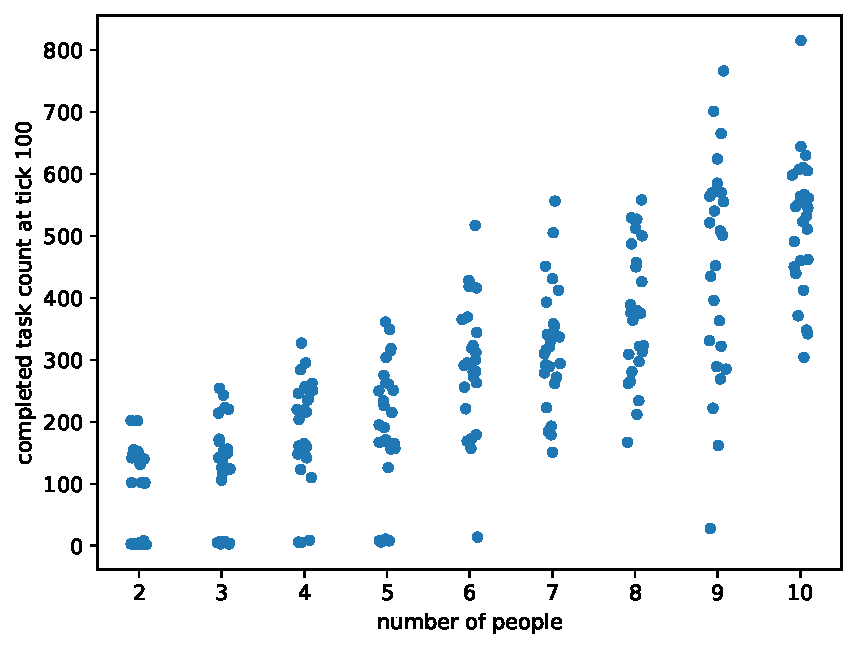
\includegraphics[width=1\textwidth]{images/task_distribution_completed_versus_size_simCount25_skills2_levels1_taskduration1_people2_social0_ticks100.pdf}
\caption{Task throughput after 100 ticks versus number of people in the organization. 25 simulations were run for each organization size. 
Adding people does increase throughput, but the variance of throughput increases due to dependence on the distribution of specializations and skill-levels of the participants. The instances where task completion is near zero occur when no members of the organization have sufficient skills to address tasks. That condition is less likely as the number of people increases.
%This configuration of the model has no social circle and the task duration is the same as the coordination duration.
}
\label{fig:task-distribution-completed-vs-size}
\end{figure}


When people in an organization are not unicorns (there are some tasks a person is unable to do), then the task throughput is lower. If an organization comprised of unicorns would operate faster, why distribute work to people who lack the skills and rely on coordination?
Because the specialization of skills is too diverse for any one person to master everything. This is easy to understand when the organization is society. It would be faster for you to 
 inspect the meat you eat for food safety, monitor the emissions of the coal-fired power plant that powers your house, build the semiconductor chips you use, and manufacture the airplane you fly. However, you don't have all those skills and you want the results quicker than you can complete the tasks yourself. Therefore, the tasks are distributed among an organization of people with different skills. The cost of coordination is that the throughput is lower.



%\subsection*{Scenario: A1,B1 or A1,B0 or A0,B1 or A0,B0\\with (task duration = coordination duration)\\with social circle}

%When a person is assigned a task they are unable to do, they spend time searching for a coworker capable of doing the task.
%The amount of time a person spends searching the organization depends on who else that person already knows. 

%If I'm qualified as ``A1" and the task is ``B1," then I can give the task to a coworker who I know is qualified as ``B1." If I don't know anyone with the relevant specialization and skill-level, then I have to search the rest of the organization.
%The more people I know the less time I spend searching.

%A person who is an A1,B1 will have no contact list because there is no handoff needed. A person who is A0,B0 will have a randomly populated contact list. A person who is A1,B0 will have a contact list populated with people who have B1.

%With this feature in the model, we can look for a tipping point when the organization is larger than the size of each member's social circle. We expect a change in throughput when the organization exceeds \href{https://en.wikipedia.org/wiki/Dunbar\%27s_number}{Dunbar's number}.

%Result: social circle size matters to throughput 
%Plot throughput versus social size for fixed organization size.




% TODO: https://en.wikipedia.org/wiki/Little%27s_law


%\subsection*{Scenario: A1,B1 or A1,B0 or A0,B1 or A0,B0\\with (task duration $>$ coordination duration)\\with no social circle}

%Result: whether throughput is lower or higher than one person is sensitive to ratio of task:coord

%Result: social circle size matters to throughput 


%\subsection*{xxx}

%A person who is an A3 B3 c3 will have no contact list because there is no handoff needed. A person who is a0 b0 c0 will have a randomly populated contact list. A person who is A3B0C0 will have a contact list populated with people who have non-zero skills in B and C

%\section{to investigate}

%The minimum throughput is no unicorns. What is the spread?

%Does the system reach steady state? 
%Or do task backlogs grow unbounded?

%What is the relevance of unicorns who can do every task well for throughput or minimum task completion time?
%(Characterization) What is the density of unicorns?




%The search time when the organization is smaller than a socialist goal is negligible, whereas when the organization is larger than their social circle the search time increases proportional to the number of people never organization. This is an obvious statement, but it indicates why larger organizations feel different than a small group of people working together who know each other.
%Hierarchy is not included in this numerical model, but it is one way of addressing this? Of how to coordinate outside of your social circle.



\section{What to Do about Too Many Tasks}

% source: https://graphthinking.blogspot.com/2023/02/prioritization-of-tasks.html

Because unicorns can do any task, one way to improve throughput is to invest in training people. Training in the context of this model has the purpose of  increased breadth (added specializations) or increased depth (improved skill-level for a specialization). One reason there are not more unicorns in an organization is that not everyone wants to know and do everything. Knowing how to create a webpage, analyze data, manage a server, initiate a contract, interact with customers, gather requirements, and run a team can feel overwhelming. Another reason unicorns are rare is turnover. When a person outgrows their assigned role,  they may look to other opportunities to feel more fulfilled. Retaining unicorns is challenging.

A separate approach to having too many tasks relative to the number of people in the workforce is to prioritize the work. Prioritization doesn't necessarily increase task throughput, but without prioritization, tasks get started and may not get completed. (The problem of ``start a task but don't finish it" isn't part of the numerical model but does happen in real organizations.)

Prioritization requires sacrifice (what tasks are you not doing) and induces risk (there are consequences to not doing tasks) and spends your reputation (not doing tasks affects other people).

There are two conditions under which prioritization becomes important:
\begin{itemize}
    \item The number of tasks is less than or equal to the amount of staff attention available and skill. Then prioritization is merely ordering the sequence of tasks.
    \item When the number of tasks exceeds staffing capacity and skill-level per person, an oversubscribed person won't get to every task. Saying no is important but harms your reputation.
\end{itemize}


Prioritization strategies options
\begin{itemize}
    \item Don't prioritize. Work on tasks as they are identified and don't complete anything because it gets interrupted by the next task
Static prioritization that is exclusive. Only work on one thing to the exclusion of everything else.
    \item Shifting prioritization (prioritization changes over time); either:
    \begin{itemize}
        \item Prioritization evolves slower than tasks can be completed.
        \item Prioritization shifts faster than tasks can be completed is ineffective because it is indistinguishable from responding to tasks as they arise.
    \end{itemize}
    \item Static prioritization by category. Likely to harm your reputation with people come to you with tasks that aren't in your primary category.
    \item Prioritization within proportionally allocated task categories. For example, suppose you have three categories of tasks. You allocate 10\% of your time to the first category, 20\% of your time to the second, and your remaining time to  the third category. 
\end{itemize}

\clearpage
\section{Software Implementation of the Simulation Model}

The model referenced in this Appendix is implemented in \href{https://en.wikipedia.org/wiki/Python_(programming_language)}{Python 3}. The primary functions used to generate data used for figures in this appendix are below. The complete source code for this book is available at \href{https://github.com/processempathy/bureaucracy-guidebook}{https://github.com/processempathy/bureaucracy-guidebook}.

The entity in this
\href{https://en.wikipedia.org/wiki/Agent-based_model}{agent-based model} is a person. For more description and context, see 
\iftoggle{haspagenumbers}{page~\pageref{sec:example-people}}{section~\ref{sec:example-people}}.
\inputminted[fontsize=\footnotesize,linenos]{python}{python3_lib_simulation__create_person.py}

The simulation depends on the following helper functions.
\inputminted[fontsize=\footnotesize,linenos]{python}{python3_lib_simulation__helper_functions.py}

\begin{landscape}
The simulation loop.
\inputminted[fontsize=\footnotesize,linenos]{python}{python3_lib_simulation__simulate.py}
\end{landscape}
